%----------
%   IMPORTANTE
%----------

% Si nunca has utilizado LaTeX es conveniente que aprendas una serie de conceptos básicos antes de utilizar esta plantilla. Te aconsejamos que leas previamente algún tutorial (puedes encontar muchos en Internet).

% Esta plantilla está basada en las recomendaciones de la guía "Trabajo fin de Grado: Escribir el TFG", que encontrarás en http://uc3m.libguides.com/TFG/escribir
% contiene recomendaciones de la Biblioteca basadas principalmente en estilos APA e IEEE, pero debes seguir siempre las orientaciones de tu Tutor de TFG y la normativa de TFG para tu titulación.

% Encontrarás un ejemplo de TFG realizado con esta misma plantilla en la carpeta "_ejemplo_TFG_2019". Consúltalo porque contiene ejemplos útiles para incorporar tablas, figuras, listados de código, bibliografía, etc.


%----------
%    CONFIGURACIÓN DEL DOCUMENTO
%----------

% Definimos las características del documento y añadimos una serie de paquetes (\usepackage{package}) que agregan funcionalidades a LaTeX.

\documentclass[12pt]{report} %fuente a 12pt

% MÁRGENES: 2,5 cm sup. e inf.; 3 cm izdo. y dcho.
\usepackage[
a4paper,
vmargin=2.5cm,
hmargin=3cm
]{geometry}

% INTERLINEADO: Estrecho (6 ptos./interlineado 1,15) o Moderado (6 ptos./interlineado 1,5)
\renewcommand{\baselinestretch}{1.15}
\parskip=6pt

\providecommand{\tightlist}{%
  \setlength{\itemsep}{0pt}\setlength{\parskip}{0pt}}

% DEFINICIÓN DE COLORES para portada y listados de código
\usepackage[table]{xcolor}
\definecolor{azulUC3M}{RGB}{0,0,102}
\definecolor{gray97}{gray}{.97}
\definecolor{gray75}{gray}{.75}
\definecolor{gray45}{gray}{.45}

\usepackage{tikz}
% Soporte para GENERAR PDF/A --es importante de cara a su inclusión en e-Archivo porque es el formato óptimo de preservación y a la generación de metadatos, tal y como se describe en http://uc3m.libguides.com/ld.php?content_id=31389625. En la carpeta incluímos el archivo plantilla_tfg_2017.xmpdata en el que puedes incluir los metadatos que se incorporarán al archivo PDF cuando lo compiles. Ese archivo debe llamarse igual que tu archivo .tex. Puedes ver un ejemplo en esta misma carpeta.
\usepackage[a-1b]{pdfx}

% ENLACES
\usepackage{hyperref}
\hypersetup{colorlinks=true,
    linkcolor=black, % enlaces a partes del documento (p.e. índice) en color negro
    citecolor=black,
    urlcolor=blue} % enlaces a recursos fuera del documento en azul

% EXPRESIONES MATEMATICAS
\usepackage{amsmath,amssymb,amsfonts,amsthm}

\usepackage{txfonts}
\usepackage[T1]{fontenc}
\usepackage[utf8]{inputenc}

\usepackage[spanish, es-tabla]{babel}
\usepackage[babel, spanish=spanish]{csquotes}
\AtBeginEnvironment{quote}{\small}

\usepackage{booktabs}

% diseño de PIE DE PÁGINA
\usepackage{fancyhdr}
\pagestyle{fancy}
\fancyhf{}
\renewcommand{\headrulewidth}{0pt}
\rfoot{\thepage}
\fancypagestyle{plain}{\pagestyle{fancy}}

% DISEÑO DE LOS TÍTULOS de las partes del trabajo (capítulos y epígrafes o subcapítulos)
\usepackage{titlesec}
\usepackage{titletoc}
\titleformat{\chapter}[block]
{\large\bfseries\filcenter}
{\thechapter.}
{5pt}
{\MakeUppercase}
{}
\titlespacing{\chapter}{0pt}{0pt}{*3}
\titlecontents{chapter}
[0pt]
{}
{\contentsmargin{0pt}\thecontentslabel.\enspace\uppercase}
{\contentsmargin{0pt}\uppercase}
{\titlerule*[.7pc]{.}\contentspage}

\titleformat{\section}
{\bfseries}
{\thesection.}
{5pt}
{}
\titlecontents{section}
[5pt]
{}
{\contentsmargin{0pt}\thecontentslabel.\enspace}
{\contentsmargin{0pt}}
{\titlerule*[.7pc]{.}\contentspage}

\titleformat{\subsection}
{\normalsize\bfseries}
{\thesubsection.}
{5pt}
{}
\titlecontents{subsection}
[10pt]
{}
{\contentsmargin{0pt}
    \thecontentslabel.\enspace}
{\contentsmargin{0pt}}
{\titlerule*[.7pc]{.}\contentspage}


% DISEÑO DE TABLAS. Puedes elegir entre el estilo para ingeniería o para ciencias sociales y humanidades. Por defecto, está activado el estilo de ingeniería. Si deseas utilizar el otro, comenta las líneas del diseño de ingeniería y descomenta las del diseño de ciencias sociales y humanidades
\usepackage{multirow} % permite combinar celdas
\usepackage{caption} % para personalizar el título de tablas y figuras
\usepackage{floatrow} % utilizamos este paquete y sus macros \ttabbox y \ffigbox para alinear los nombres de tablas y figuras de acuerdo con el estilo definido. Para su uso ver archivo de ejemplo
\usepackage{array} % con este paquete podemos definir en la siguiente línea un nuevo tipo de columna para tablas: ancho personalizado y contenido centrado
\newcolumntype{P}[1]{>{\centering\arraybackslash}p{#1}}
\DeclareCaptionFormat{upper}{#1#2\uppercase{#3}\par}

% Diseño de tabla para ingeniería
\captionsetup[table]{
    format=upper,
    name=TABLA,
    justification=centering,
    labelsep=period,
    width=.75\linewidth,
    labelfont=small,
    font=small,
}

%Diseño de tabla para ciencias sociales y humanidades
%\captionsetup[table]{
%    justification=raggedright,
%    labelsep=period,
%    labelfont=small,
%    singlelinecheck=false,
%    font={small,bf}
%}


% DISEÑO DE FIGURAS. Puedes elegir entre el estilo para ingeniería o para ciencias sociales y humanidades. Por defecto, está activado el estilo de ingeniería. Si deseas utilizar el otro, comenta las líneas del diseño de ingeniería y descomenta las del diseño de ciencias sociales y humanidades
\usepackage{graphicx}
\graphicspath{{imagenes/}} %ruta a la carpeta de imágenes

% Diseño de figuras para ingeniería
\captionsetup[figure]{
    format=hang,
    name=Fig.,
    singlelinecheck=off,
    labelsep=period,
    labelfont=small,
    font=small
}

% Diseño de figuras para ciencias sociales y humanidades
%\captionsetup[figure]{
%    format=hang,
%    name=Figura,
%    singlelinecheck=off,
%    labelsep=period,
%    labelfont=small,
%    font=small
%}


% NOTAS A PIE DE PÁGINA
\usepackage{chngcntr} %para numeración contínua de las notas al pie
\counterwithout{footnote}{chapter}

% LISTADOS DE CÓDIGO
% soporte y estilo para listados de código. Más información en https://es.wikibooks.org/wiki/Manual_de_LaTeX/Listados_de_código/Listados_con_listings
\usepackage{listings}

% definimos un estilo de listings
\lstdefinestyle{estilo}{ frame=Ltb,
    framerule=0pt,
    aboveskip=0.5cm,
    framextopmargin=3pt,
    framexbottommargin=3pt,
    framexleftmargin=0.4cm,
    framesep=0pt,
    rulesep=.4pt,
    backgroundcolor=\color{gray97},
    rulesepcolor=\color{black},
    %
    basicstyle=\ttfamily\footnotesize,
    keywordstyle=\bfseries,
    stringstyle=\ttfamily,
    showstringspaces = false,
    commentstyle=\color{gray45},
    %
    numbers=left,
    numbersep=15pt,
    numberstyle=\tiny,
    numberfirstline = false,
    breaklines=true,
    xleftmargin=\parindent
}

\captionsetup[lstlisting]{font=small, labelsep=period}
% fijamos el estilo a utilizar
\lstset{style=estilo}
\renewcommand{\lstlistingname}{\uppercase{Código}}


%BIBLIOGRAFÍA - PUEDES ELEGIR ENTRE ESTILO IEEE O APA. POR DEFECTO ESTÁ CONFIGURADO IEEE. SI DESEAS USAR APA, COMENTA LAS LÍNEA DE IEEE Y DESCOMENTA LAS DE APA. Si haces cambios en la configuración de la bibliografía y no obtienes los resultados esperados, es recomendable limpiar los archivos auxiliares y volver a compilar en este orden: COMPILAR-BIBLIOGRAFIA-COMPILAR

% Tienes más información sobre cómo generar bibliografía y CONFIGURAR TU EDITOR DE TEXTO para compilar con biber en http://tex.stackexchange.com/questions/154751/biblatex-with-biber-configuring-my-editor-to-avoid-undefined-citations , https://www.overleaf.com/learn/latex/Bibliography_management_in_LaTeX y en http://www.ctan.org/tex-archive/macros/latex/exptl/biblatex-contrib
% También te recomendamos consultar la guía temática de la Biblioteca sobre citas bibliográficas: http://uc3m.libguides.com/guias_tematicas/citas_bibliograficas/inicio

% CONFIGURACIÓN PARA LA BIBLIOGRAFÍA IEEE
\usepackage[backend=biber, style=ieee, isbn=false,sortcites, maxbibnames=5, minbibnames=1]{biblatex} % Configuración para el estilo de citas de IEEE, recomendado para el área de ingeniería. "maxbibnames" indica que a partir de 5 autores trunque la lista en el primero (minbibnames) y añada "et al." tal y como se utiliza en el estilo IEEE.

%CONFIGURACIÓN PARA LA BIBLIOGRAFÍA APA
%\usepackage[style=apa, backend=biber, natbib=true, hyperref=true, uniquelist=false, sortcites]{biblatex}
%\DeclareLanguageMapping{spanish}{spanish-apa}

% Añadimos las siguientes indicaciones para mejorar la adaptación de los estilos en español
\DefineBibliographyStrings{spanish}{%
    andothers = {et\addabbrvspace al\adddot}
}
\DefineBibliographyStrings{spanish}{
    url = {\adddot\space[En línea]\adddot\space Disponible en:}
}
\DefineBibliographyStrings{spanish}{
    urlseen = {Acceso:}
}
\DefineBibliographyStrings{spanish}{
    pages = {pp\adddot},
    page = {p.\adddot}
}

\addbibresource{bibliografia/bibliografia.bib} % llama al archivo bibliografia.bib en el que debería estar la bibliografía utilizada


%-------------
%    DOCUMENTO
%-------------

\begin{document}
\pagenumbering{roman} % Se utilizan cifras romanas en la numeración de las páginas previas al cuerpo del trabajo

%----------
%    PORTADA
%----------
\title{Práctica 2}
\author{Álvaro Guerrero Espinosa (100472294)\\
        César López Mantecón (100472092)\\
        Paula Subías Serrano (100472119)\\
        Irene Subías Serrano (100472108)\\}

\makeatletter
\begin{titlepage}
    \begin{sffamily}
    \color{azulUC3M}
    \begin{center}
        \begin{figure}[H] %incluimos el logotipo de la Universidad
            \makebox[\textwidth][c]{
\includegraphics[width=16cm]{Portada_Logo.png}}
        \end{figure}
        \vspace{2.5cm}
        \begin{Large}
            Grado en Ingeniería Informática\\
            \@date\\
            \vspace{2cm}
            \textsl{Inteligencia Artificial en las Organizaciones}\\
            \bigskip
        \end{Large}
        {\Huge ``\@title''}\\
        \vspace*{0.5cm}
        \rule{10.5cm}{0.1mm}\\
        \vspace*{0.9cm}
        {\LARGE\@author}
        \vspace*{1cm}
    \end{center}
    \vfill
    \color{black}
    % si nuestro trabajo se va a publicar con una licencia Creative Commons, incluir estas líneas. Es la opción recomendada.
    
\includegraphics[width=4.2cm]{imagenes/creativecommons.png}\\ %incluimos el logotipo de creativecommons
    Esta obra se encuentra sujeta a la licencia Creative Commons \textbf{Reconocimiento - No Comercial - Sin Obra Derivada}
    \end{sffamily}
\end{titlepage}
\makeatother

\newpage %página en blanco o de cortesía
\thispagestyle{empty}
\mbox{}

%----------
%    ÍNDICES
%----------

%--
% Índice general
%-
\tableofcontents
\thispagestyle{fancy}

\newpage % página en blanco o de cortesía
\thispagestyle{empty}
\mbox{}

%--
% Índice de figuras. Si no se incluyen, comenta las líneas siguientes
%-
 \listoffigures
 \thispagestyle{fancy}

 \newpage % página en blanco o de cortesía
 \thispagestyle{empty}
 \mbox{}

%--
% Índice de tablas. Si no se incluyen, comenta las líneas siguientes
%-
\listoftables
 \thispagestyle{fancy}

 \newpage % página en blanco o de cortesía
 \thispagestyle{empty}
 \mbox{}


%----------
%    TRABAJO
%----------
\clearpage
\pagenumbering{arabic} % numeración con múmeros arábigos para el resto de la publicación
% TODO: redactar introducción
% TODO: captions
% Para cada atributo: significado, rango, (si numero) min/max/media/moda, (si categorico) desbalanceo, missing values


\chapter{Introducción}
\label{chap:intro}

\chapter{Análisis exploratorio de los datos (EDA)}
\label{chap:eda}
El \textit{dataset} cuenta con 3411 instancias de reseñas a vuelos. Para cada reseña se incluyen 19 atributos de distinta naturaleza: campos textuales, fechas, datos categóricos y datos numéricos. A continuación haremos un breve repaso por cada uno de los atributos, explorando su tipo, su significado y el número de valores faltantes.

\begin{itemize}
    \item \textbf{Airline Name:} representa el nombre de la aerolínea asociado al vuelo reseñado. Se trata de un atributo \textit{nominal}.
    \item \textbf{Aircraft:} representa el modelo de avión empleado en el vuelo reseñado. Se trata de un atributo \textit{nominal}.  
    \item \textbf{Cabin Staff Service:} puntuación numérica del 0 al 50 sobre el servicio del personal a bordo. Se trata de un atributo \textit{numérico}. Cabe destacar que los valores que toma son siempre múltiplos de 10.
    \item \textbf{Date Flown:} fecha en la que se realizó el vuelo.
    \item \textbf{Food \& Beverages:} puntuación numérica del 0 al 50 sobre el servicio de comida en el vuelo. Se trata de un atributo \textit{numérico}. Cabe destacar que los valores que toma son siempre múltiplos de 10. 
    \item \textbf{Ground Service:} puntuación numérica del 0 al 50 sobre el servicio en tierra. Se trata de un atributo \textit{numérico}. Cabe destacar que los valores que toma son siempre múltiplos de 10.
    \item \textbf{Inflight Entertainment:} puntuación numérica del 0 al 50 sobre el servicio de entretenimiento durante el vuelo. Se trata de un atributo \textit{numérico}. Cabe destacar que los valores que toma son siempre múltiplo sde 10.
    \item \textbf{Overall Rating:} puntuación numérica del 1 al 9. Representa el grado de satisfacción del cliente. Se trata de un atrbito \textit{numérico}. Además, se trata de nuestra \textbf{variable objetivo}.
    \item \textbf{Recomended:} valor \textit{booleano}. Representa si el cliente recomendaría el servicio. Destaca un desbalanceo del 69.95\% hacia el valor negativo.
    \item \textbf{Review:} atributo \textit{textual}. Contiene el comentario del usuario sobre el vuelo.
    \item \textbf{Review Date:} fecha en la que se realizó la reseña.
    \item \textbf{Review Title:} campo \textit{texual}. Da título a la reseña. 
    \item \textbf{Route:} campo \textit{textual}. Representa la ruta del vuelo.
    \item \textbf{Seat Comfort:} puntuación numérica del 0 al 50 sobre la comodidad de los asientos. Se trata de un atributo \textit{numérico}. Cabe destacar que los valores que toma son siempre múltiplo sde 10.
    \item \textbf{Seat Type:} atributo \textit{nominal}. Describe el tipo de asiento. Puede tomar los valores ``Ecoclass'',  ``Business Class'', ``Premium Economy'' y ``First Class''.  
    \item \textbf{Type Of Traveller:} atributo \textit{nominal}. Representa el tipo de viajero. Puede tomar los valores ``Solo Leisure'', ``Couple Leisure'', ``Family Leisure'' y ``Business''.
    \item \textbf{Value For Money:} puntuación numérica del 0 al 50 sobre el valor percibido con respecto al dinero gastado. Se trata de un atributo \textit{numérico}. Cabe destacar que los valores que toma son siempre múltiplo sde 10.
    \item \textbf{Verified:} atributo \textit{booleano}. Representa si la persona que realiza la reseña está verificada. Ambas clases están balanceadas, con un 55.77\% de inclinación hacia la clase mayoritaria.
    \item \textbf{Wifi \& Connectivity:} puntuación numérica del 0 al 50 sobre la conexión a internet durante el vuelo. Se trata de un atributo \textit{numérico}. Cabe destacar que los valores que toma son siempre múltiplo sde 10.
\end{itemize}
En la siguientes tablas se recogen los datos relevantes para cada atributo: 
\begin{table}[H]
    \begin{center}
        \begin{tabular}{@{}cccccc@{}}
            \toprule
            Atributo & Airline Name       & Aircraft & Cabin Staff Service & Date Flown & Food \& Beverages \\ 
            \midrule
            Tipo     & Nominal            & Nominal  & Numérico            & Fecha      & Numérico          \\ 
            Min      & -                  & -        & 0                   & 04/01/2012 & 0                 \\ 
            Max      & -                  & -        & 50                  & 07/01/2023 & 50                \\ 
            Media    & -                  & -        & 26.259              & -          & 23.298            \\ 
            Moda     & Tigerair Australia & A320     & 10                  & 05/01/2023 & 10                \\ 
            missing (\%) & 0              & 70.57\%  & 16.82\%             & 11.83\%    & 38.15\%           \\ 
            \bottomrule
        \end{tabular} 
        \caption{Datos de los atributos - 1}
    \end{center}
\end{table}

\begin{table}[H]
    \begin{center}
        \begin{tabular}{@{}cccccc@{}}
            \toprule
            Atributo & Ground service & Infight Entertainment & Overall Rating & Recommended & Review  \\ 
            \midrule
            Tipo     & Numérico       & Numérico              & Numérico       & Booleano    & Textual \\ 
            Min      & 10             & 0                     & 1              & -           & -       \\ 
            Max      & 50             & 50                    & 9              & -           & -       \\ 
            Media    & 20.646         & 19.792                & 3.368          & -           & -       \\ 
            Moda     & 10             & 10                    & 1              & NO        & -       \\ 
            missing (\%) & 17.32\%    & 53.10\%               & 0\%            & 0\%         & -       \\ 
            \bottomrule
        \end{tabular} 
        \caption{Datos de los atributos - 2}
    \end{center}
\end{table}
\begin{table}[H]
    \begin{center}
        \begin{tabular}{@{}cccccc@{}}
            \toprule
            Atributo & Review Date & Review Title & Route   & Seat Confort & Seat Type    \\ 
            \midrule
            Tipo     & Fecha       & Textual      & Nominal & Numérico     & Nominal      \\ 
            Min      & 03/06/2004  & -            & -       & 0            & -            \\ 
            Max      & 27/07/2023  & -            & -       & 50           & -            \\ 
            Media    &             & -            & -       & 23.831       & -            \\ 
            Moda     & 16/07/2023  & -            & -       & 10           & Economy Class\\ 
            missing (\%) & 0    \% & 0\%          & 12.22\% & 16.28\%      & 1.71\%       \\ 
            \bottomrule
        \end{tabular} 
        \caption{Datos de los atributos - 3}
    \end{center}
\end{table}
\begin{table}[H]
    \begin{center}
        \begin{tabular}{@{}ccccc@{}}
            \toprule
            Atributo & Type of Traveller & Value For Money & Verified  & Wifi \& Connectivity \\ 
            \midrule
            Tipo     & Nominal           & Numérico        & Booleano  & Numérico             \\ 
            Min      & -                 & 0               & -         & 10                   \\ 
            Max      & -                 & 50              & -         & 50                   \\ 
            Media    &                   & 22.050          & -         & 15.338               \\ 
            Moda     & Solo Leisure      & 10              & Verdadero & 10                   \\ 
            missing (\%) & 11.79\%       & 0\%             & 0\%       & 72.69\%              \\ 
            \bottomrule
        \end{tabular} 
        \caption{Datos de los atributos - 4}
    \end{center}
\end{table}

\chapter{Preprocesado}
\label{chap:preprocess}
En este capítulo se describen las diferentes transformaciones aplicadas a los datos para su ponsterior uso en el entrenamiento de modelos.

\section{Eliminación de atributos}
\label{sec:delete_columns}
Se han seguido 3 criterios para la eliminación de atributos:
\begin{itemize}
    \item Relevancia: algunos datos no aportan información relevante de cara al entrenamiento del modelo. Por este criterio se han eliminado \textit{Date Flown} y \textit{Date Review}.
    \item Afectar negativamente al modelo: algunos atributos nominales cuentan con un número de clases muy numeroso. En el caso de \textit{Route}, tratar con todas ellas añade una gran complejidad que no se traducía a un mejor rendimiento. En consecuencia, se ha eliminado este atributo. 
    \item Numerosos valores faltantes: se han eliminado todos los atributos con un número de \textit{missing values} superior al 35\% de los valores totales. Esto es porque se considera que no contamos con información suficiente para imputar estos datos.
\end{itemize}
A continuación se muestra un gráfico con el número de valores faltantes por atributo:

\begin{figure}[H]
    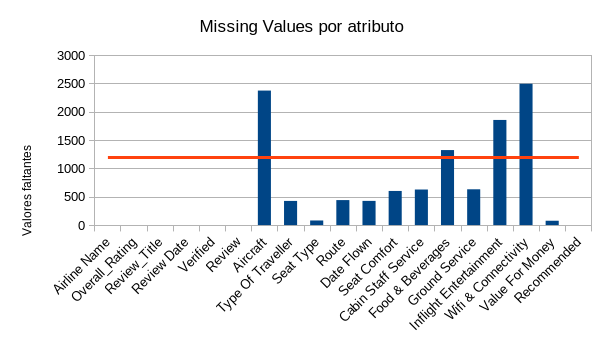
\includegraphics[width=0.85\linewidth]{missings.png}\\ 
    \caption{Número de valores faltantes por atributo}
\end{figure}

La línea sobre el gráfico señala el 35\% de las instancias.

\section{Formateo de los datos}
\label{sec:formateo}
Se han sustituído los valores de las columnas booleanas (i.e. \textit{Verified} y \textit{Recommended}) por valores binarios. Los valores nominales se han codificado a través mediante \textit{One-hot encoding}, a excepción de \textit{Airline} (esto es por limitaciones de la implementación). Los atributos codificados a través de \textit{OHE} han sido: \textit{Seat Type} y \textit{Type of Traveller}.

\section{Imputación de valores faltantes}
\label{sec:imputacion}

\chapter{Modelo básico sin usar datos textuales}
\label{chap:basicModel}

\chapter{Proceso de entrenamiento}
\label{chap:train}

\section{Parte 1 - Modelado sin análisis de sentimientos}
\label{sec:parte1}

\section{Parte 2 - Modelado con análisis de sentimientos}
\label{sec:parte2}

\chapter{Comparación de resultados}
\label{chap:resultados}

\chapter{Conclusión}
\label{chap:conclusion}

Esta práctica nos ha permitido explorar nuevas técnicas para la construcción de modelos. En concreto, hemos podido comprobar como el \textit{text mining} presenta grandes ventajas frente a modelos que no aprovechan toda la información contenida en campos de texto.

Además, el análisis de sentimientos ha demostrado ser de gran utilidad en esta clase de aplicaciones. Conocer el sentimiento de un agente hacia un dominio mediante el análisis de datos tiene muy buenas aplicaciones en el campo del marketing y el análisis empresarial.
%----------
%    BIBLIOGRAFÍA
%----------

%\nocite{*} % Si quieres que aparezcan en la bibliografía todos los documentos que la componen (también los que no estén citados en el texto) descomenta está lína

\clearpage

\phantomsection
\addcontentsline{toc}{chapter}{Bibliografía}
\label{chap:bibliography}
\setquotestyle[english]{british} % Cambiamos el tipo de cita porque en el estilo IEEE se usan las comillas inglesas.
\printbibliography



%----------
%    ANEXOS
%----------

% Si tu trabajo incluye anexos, puedes descomentar las siguientes líneas
%\chapter* {Anexo x}
%\pagenumbering{gobble} % Las páginas de los anexos no se numeran



\end{document}
